\documentclass[10pt]{beamer}
\usetheme{metropolis}           % Use metropolis theme
\title{Smart data}
\subtitle{Soutenance de stage - 2 juillet 2018}
\date{Master 1 Classique MIAGE,\\
Accueilli par FRS Consulting
}
\author{Alexandre Petit-Pas}
\institute{Tuteur : Dr. Gaétan Le Chat\\ Référent : Prof. Pascal Poizat}
\logo{
\includegraphics[scale=0.1]{resources/frs.png}}

\usepackage{FiraSans}
\usepackage{xcolor}
\usepackage{appendix}
\usepackage{animate}
\usepackage{booktabs}
\usepackage{array}
\definecolor{frsblue}{HTML}{004475} %R:0 G:68 B:117
\definecolor{lightgray}{HTML}{D3D3D3}

\metroset{
	numbering=fraction
}
\titlegraphic{
	\vspace{3.5cm}\hfill
	
\includegraphics[scale=0.7]{resources/logos.png}	
}


\setbeamercolor{frametitle}{fg=white, bg=frsblue}
\setbeamercolor{title}{fg=frsblue}
\setbeamercolor{progress bar}{fg=frsblue, bg=lightgray}
\setbeamercolor{title separator}{fg=frsblue, bg=lightgray}
\setbeamercolor{progress bar in head/foot}{fg=frsblue, bg=lightgray}
\setbeamercolor{progress bar in section page}{fg=frsblue, bg=lightgray}

\setbeamertemplate{footline}[text line]{%
  \parbox{\linewidth}{\color{frsblue}\vspace*{-8pt}\insertsubtitle\hfill\inserttitle\hfill\insertsectionhead\hfill\insertpagenumber}}

\begin{document}
	\maketitle
	\section{Cadre du stage}
		\begin{frame}{FRS Consulting}
			\begin{figure}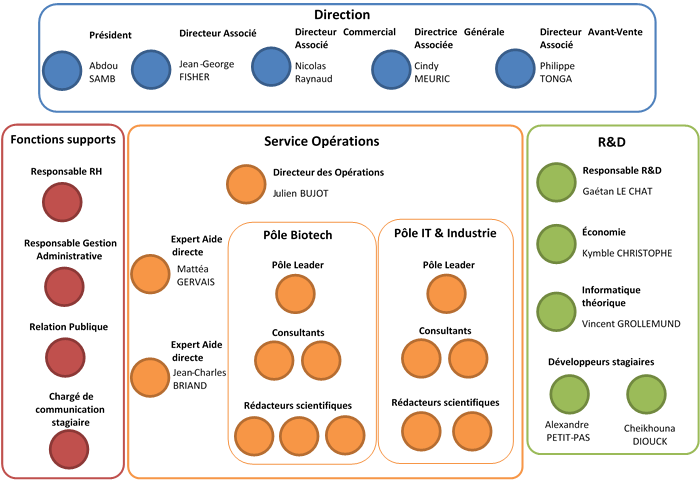
\includegraphics[width=\linewidth]{resources/organigramme.png}\end{figure}
		\end{frame}
		\begin{frame}{finElink}
			\begin{minipage}[c]{0.49\linewidth}
				\begin{figure}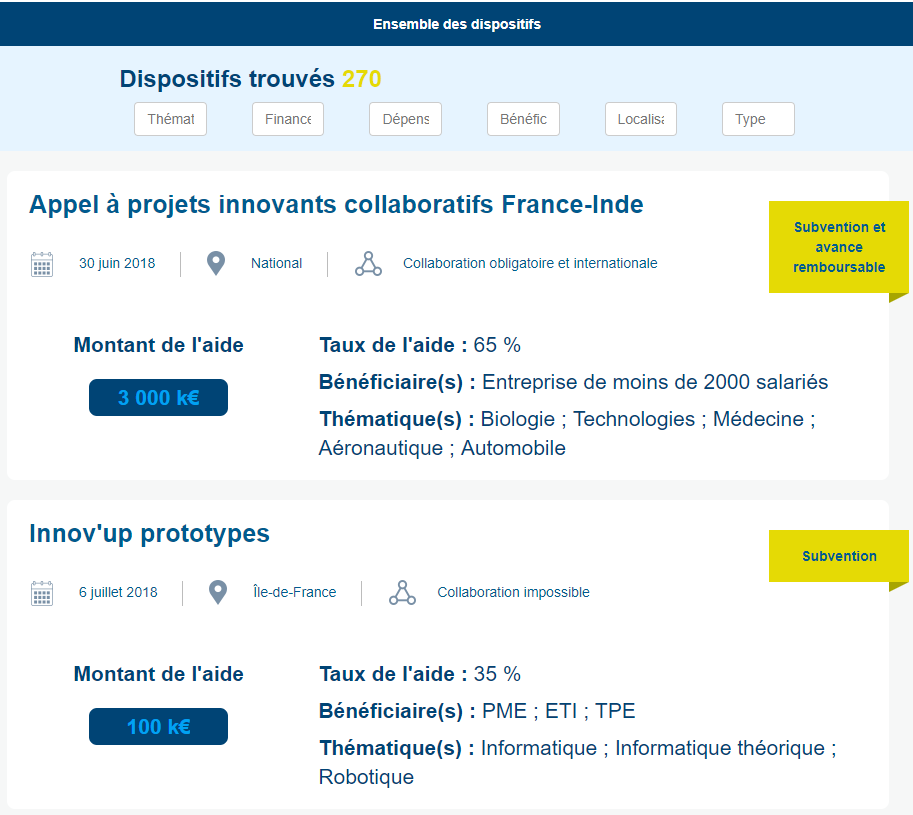
\includegraphics[height=4cm, width=\linewidth]{resources/finelink2.png}\caption{Annuaire}\end{figure}
 			\end{minipage}
 			\begin{minipage}[c]{0.49\linewidth}
 					\begin{figure}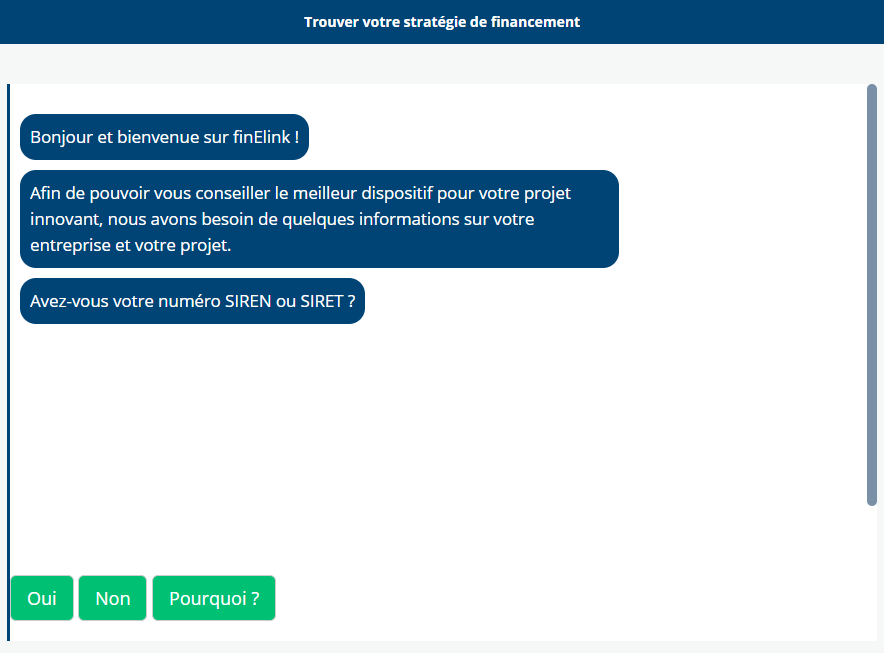
\includegraphics[height=4cm, width=\linewidth]{resources/finelink1.png}\caption{Recommandation}\end{figure}
			\end{minipage}
		\end{frame}
		\begin{frame}{Business Explorer}
		 \begin{figure}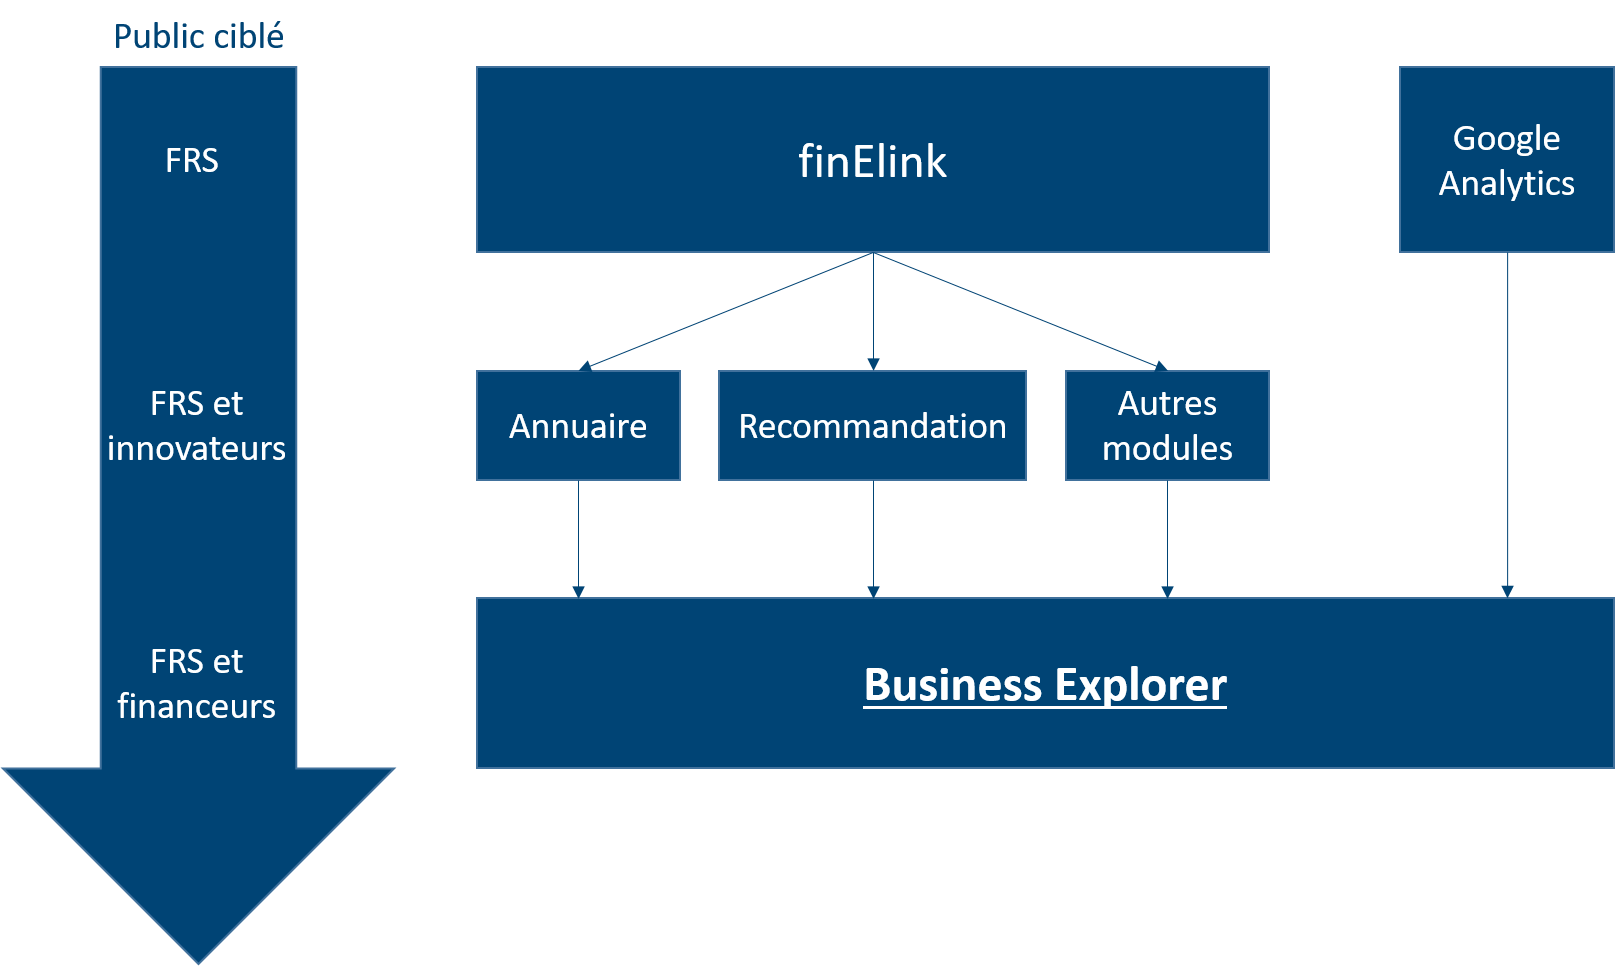
\includegraphics[width=\linewidth]{resources/businessexplorer.png}\end{figure}
		\end{frame}
			
	\section{Méthodologies}
	\begin{frame}{Gestion du projet}
		\begin{figure}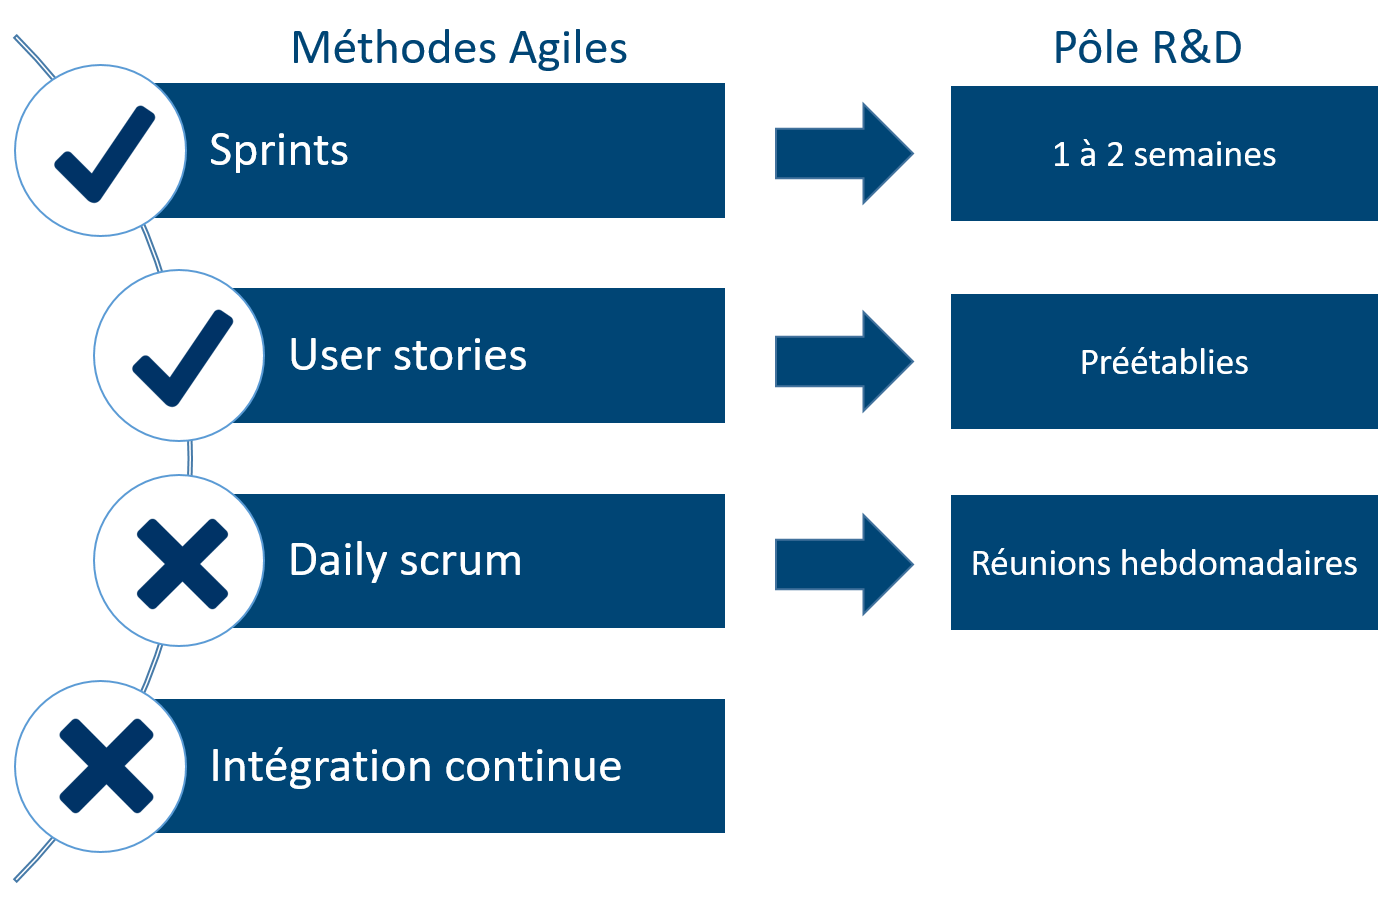
\includegraphics[width=\linewidth]{resources/methodologies.png}\end{figure}
	\end{frame}
	\begin{frame}{Organisation du travail}
	\begin{figure}
	 \begin{center}
	 	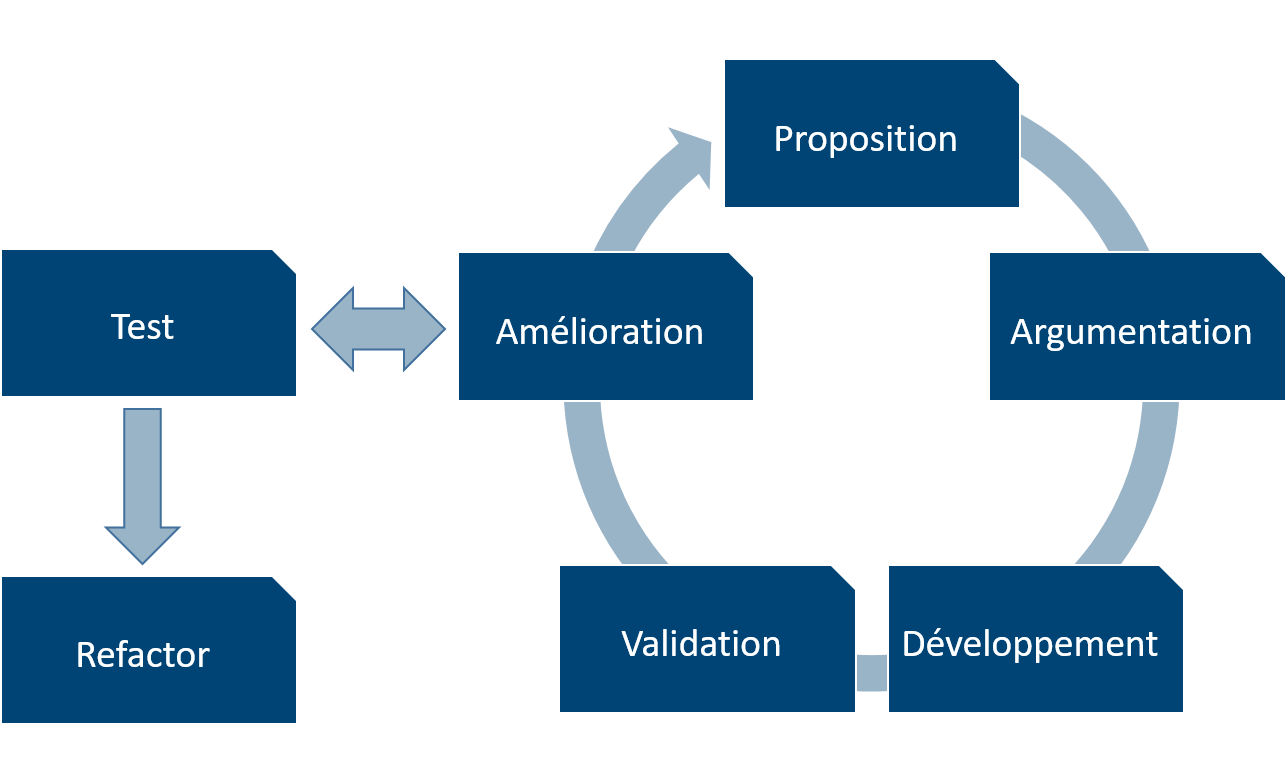
\includegraphics[scale=0.4]{resources/travail.png}
	 \end{center}
	 \end{figure}
	\end{frame}
	\section{Réalisations}
		\begin{frame}{Benchmark}
			\begin{figure}
			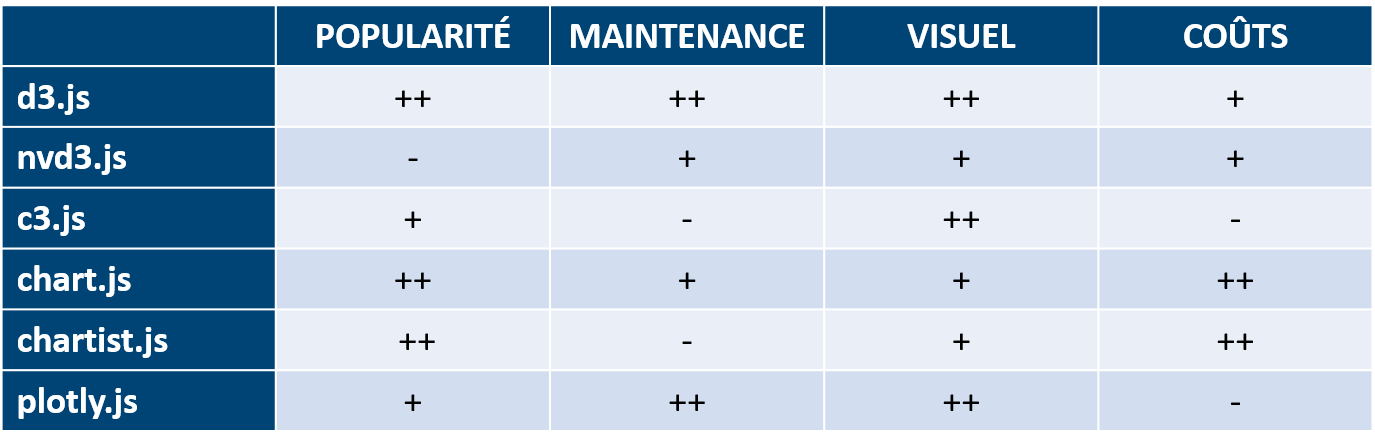
\includegraphics[width=\linewidth]{resources/bench.png}
			\end{figure}
		\end{frame}
		\begin{frame}{Sunburst}
			\animategraphics[loop,controls,buttonsize=0.2cm,width=\linewidth]{10}{resources/gif/sunburst-}{0}{91}
		\end{frame}
	\section{Réflexions}
	\begin{frame}{Améliorations et évolutions}
	\begin{itemize}[<+- | alert@+>]
	\item Amélioration de la couverture du code
	\item Bêta testeurs
	\item Valorisation des dispositifs unitairement
	\item Valorisation des projets
	\end{itemize}
	\end{frame}
	\begin{frame}{Bilan personnel}
	\begin{center}
	\begin{figure}
	
\includegraphics[scale=2]{resources/dataviz.png}	
	\end{figure}
	\end{center}
 	\end{frame}
\end{document}